\documentclass[format=acmsmall, review=false, screen=true]{acmart}
\settopmatter{printacmref=false} % Removes citation information below abstract
\renewcommand\footnotetextcopyrightpermission[1]{} % removes footnote with conference information in first column
\pagestyle{plain} % removes running headers
\acmYear{2018}
\acmMonth{3}

\usepackage[utf8]{inputenc}
\usepackage{microtype}
\usepackage{amsmath}
\usepackage{listings}
\usepackage{amsmath}
\usepackage{float}
\usepackage{wrapfig}
\usepackage{subcaption}
\usepackage{dirtytalk}

\lstset{
  basicstyle=\ttfamily,
  columns=fullflexible,
  frame=single,
  breaklines=true,
  postbreak=\mbox{\textcolor{red}{$\hookrightarrow$}\space},
  aboveskip=10pt,
  belowskip=5pt,
  tabsize=2
} 

\setlength{\textfloatsep}{14pt}
\setlength{\abovecaptionskip}{4pt}
\setlength{\belowcaptionskip}{4pt}

\author{Richard Bányi}


\title{\textsc{PCPP} - Reexam 2017}
\subtitle{\textsc{IT University of Copenhagen, Autumn 2017}}
\acmDOI{}
\begin{document}
\maketitle 

\section{Question 1}

What I have witnessed is that the Ser Sort performs that the worse from all of the other algorithms. The execution time is best for the SerCountRC, SerCountIt where the size of the throughput does not really affects the execution time.

\begin{figure}
  \includegraphics[width=0.7\textwidth]{benchmark.png}
  \caption{Benchmark Test \textit{BenchMark}}
  \label{fig:benchmark}
\end{figure}

\textit{Implementation - TestQuickSelect.java}

I have parallelized \textit{quickCountRec()}  see the \textit{quickCountParRec()} method.
I have used tasks, as the exam outlined I divide the array equally into regions \textit{Ai} each task get's a portion of the array and counts the number \textit{si} of elements which are smaller then the pivot in the region \textit{Ai}. The \textit{counter} is local to every thread, therefore there is no need for synchronization and also there is no shared mutate state, since all threads are working on a different region of \textit{Ai}. Afterwards I sum up all the local count of each thread which than tells which direction we need to filter.

Given this information, similarly the filtering of the regions is divided into different tasks. Because of the indexing of regions and for the sake of the implementation simplicity, each tasks has it's own local array where the filtering is happening and in the end each local array is concatenated in order. However this might not be an optimal solution and a more clever solution could be implemented by keeping the counts of each region at the counting stage.

\textit{parallel-quickCountRec vs ser-countIt}

\begin{lstlisting}[language=java]
	# OS:   Mac OS X; 10.13.3; x86_64
	# JVM:  Oracle Corporation; 1.8.0_144
	# CPU:  null; 8 "cores"
	# Date: 2018-03-01T13:20:31+0100
parallel-countRc               100 4            13.4 ns      15.02       1024
parallel-countRc               200 4            22.8 ns      25.52        512
parallel-countRc               400 4            58.9 ns      65.92        256
parallel-countRc               800 4            46.6 ns      52.10        256
parallel-countRc              1600 4           336.6 ns     376.29         32
parallel-countRc              3200 4           194.4 ns     217.38         64
parallel-countRc              6400 4          1463.5 ns    1636.33          8
parallel-countRc             12800 4          9903.6 ns   12897.89          2
parallel-countRc             25600 4         25587.4 ns   28618.43          2
parallel-countRc             51200 4          9046.8 ns   10117.24          2
ser-countIt                    100 1            36.2 ns      40.50     524288
ser-countIt                    200 1            79.5 ns      88.90      65536
ser-countIt                    400 1           183.0 ns     204.62      16384
ser-countIt                    800 1           332.8 ns     372.14       4096
ser-countIt                   1600 1           606.7 ns     678.33       2048
ser-countIt                   3200 1          1147.5 ns    1282.91        512
ser-countIt                   6400 1          2261.7 ns    2528.89        128
ser-countIt                  12800 1          4551.1 ns    5088.37         32
ser-countIt                  25600 1          9282.8 ns   10379.30          8
ser-countIt                  51200 1         18593.7 ns   20789.94          2
\end{lstlisting}

We can witness that the parallel implementation \textit{parallel-quickCountRec} is almost 3 times faster than the serial one. We can see that creating more than 4-5 tasks does not lead to better performance. The best results have been achieved with 4 tasks. 

\textit{Parallel solution - benchmarking for different number of tasks.}

\begin{lstlisting}[language=java]
parallel-countRc            500000   1          1028.8 ns    1150.52          4
parallel-countRc            500000   2           726.8 ns     812.71          4
parallel-countRc            500000   3           584.7 ns     653.69          4
parallel-countRc            500000   4           586.5 ns     655.80          4
parallel-countRc            500000   5           643.7 ns     719.68          4
parallel-countRc            500000   6           602.7 ns     673.97          4
parallel-countRc            500000   7           651.2 ns     728.48          4
parallel-countRc            500000   8           639.2 ns     714.62          4
parallel-countRc            500000   9           595.5 ns     665.83          4
parallel-countRc            500000  10           595.9 ns     666.22          4
parallel-countRc            500000  11           661.6 ns     739.71          4
parallel-countRc            500000  12           648.3 ns     724.80          4
parallel-countRc            500000  13           628.7 ns     702.88          4
parallel-countRc            500000  14           624.8 ns     698.60          4
parallel-countRc            500000  15           621.3 ns     694.66          4
parallel-countRc            500000  16           667.8 ns     746.60          4
parallel-countRc            500000  17           664.9 ns     743.42          4
parallel-countRc            500000  18           678.7 ns     758.79          4
parallel-countRc            500000  19           650.5 ns     727.39          4
parallel-countRc            500000  20           647.0 ns     723.43          4
parallel-countRc            500000  21           659.0 ns     737.03          4
parallel-countRc            500000  22           645.7 ns     722.00          4
parallel-countRc            500000  23           730.5 ns     816.77          4
parallel-countRc            500000  24           716.1 ns     800.75          4
parallel-countRc            500000  25           717.9 ns     802.95          4
parallel-countRc            500000  26           729.8 ns     815.98          4
parallel-countRc            500000  27           749.2 ns     837.63          4
parallel-countRc            500000  28           740.0 ns     827.41          4
parallel-countRc            500000  29           721.8 ns     807.15          4
parallel-countRc            500000  30           726.7 ns     812.91          4
parallel-countRc            500000  31           729.0 ns     815.16          4
parallel-countRc            500000  32           722.7 ns     808.11          4
\end{lstlisting}


\section{Question 2}

Implementation can be find in the files, however I was unable to implement it proberly due to stackoveflow errors.

\section{Question 3}

Oral discussion.

\section{Question 4}

\subsection{Why is this implementation dead-lock prone?}

The implementation is dead-lock prone because of the lack of consistent lock coordination.
In fact a thread acquires two locks but it does not pick the locations of the elements in a deterministic order. Therefore it might happen that 2 threads trying to acquire the same locks but in opposite directions making them block each other.

\subsection{Give an example program using this data structure and a schedule that deadlocks.}

Thread A comes and acquires the lock at index 7 and between acquiring the second lock at index 10 B thread is scheduled and acquires the lock at index 10, therefore 10 is locked and thread A cannot progress, and either B because it's trying to acquire the lock at index 7 that is being hold by thread A. Thus they're trying to acquiring the same lock and are in dedlock now.

\begin{lstlisting}[language=java]
synchronized (nodes[rx]) {
    // A thread acquires lock on 7 and wants to acquire the lock on 10
    // however between the synchronized methods B threads comes in and
    // acquires the lock on 10 and wants to acquire the lock on 7 which
    // is beaing hold by thread A.
    synchronized (nodes[ry]) {...}
\end{lstlisting}

\subsection{Implement a test program that uses the above data structure and provokes a deadlock with reasonable probability and run it. Do you see it deadlocking? Discuss your findings.}

\begin{lstlisting}[language=java]
  public void deadlockTest(int x, int y, final UnionFind uf) throws Exception {
    System.out.printf("Testing %s ... ", uf.getClass());
    final int threadCount = 32;
    final CyclicBarrier startBarrier = new CyclicBarrier(threadCount*2),
      stopBarrier = startBarrier;
      for (int i = 0; i < threadCount; ++i) {
        Thread ti = new Thread(new Runnable() { public void run() {
          try { startBarrier.await(); } catch (Exception exn) { }
            uf.union(x, y);
          try { stopBarrier.await(); } catch (Exception exn) { }
        }});
        Thread tj = new Thread(new Runnable() { public void run() {
          try { startBarrier.await(); } catch (Exception exn) { }
            uf.union(y, x);
          try { stopBarrier.await(); } catch (Exception exn) { }
        }});
        ti.start();
        tj.start();
      }
      startBarrier.await();
      stopBarrier.await();
      System.out.println("passed");
  }
}
\end{lstlisting}

In order for deadlock scheduling to happen as I have described in the previous question I have run many threads sequentially and tested that on my machine I had to increase the number of threads to ensure the bigger likelihood of deadlocking.

\textit{Results with 8 threads.}

\begin{lstlisting}[language=java]
Testing class CoarseUnionFind ... passed
Testing class FineUnionFind ... passed
Testing class WaitFreeUnionFind ... passed
Testing class BogusFineUnionFind ... passed
\end{lstlisting}

\textit{Results with 16 threads.}

\begin{lstlisting}[language=java]
Testing class CoarseUnionFind ... passed
Testing class FineUnionFind ... passed
Testing class WaitFreeUnionFind ... passed
Testing class BogusFineUnionFind ... deadlock
\end{lstlisting}

\section{Question 5}

\subsection{LinnkedListStack}

\textit{Implementation: ConcurrentStack.java}

The implementation follows the Java monitor pattern: all mutable fields are private,
all public methods are synchronized, and no internal data structures escapes.

For the correctness of the functional requirements I have created a very
basic single-threaded functional testing while implementing the stack based
linked list, the method name is called \textit{seqTest}.

\begin{lstlisting}[language=java]
private static void seqTest(final ConcurrentStackImp stack) {
  System.out.printf("Sequential test %n%s%n", stack.getClass());

  assert stack.size() == 0;
  stack.push(1);
  stack.push(2);
  assert stack.size() == 2;
  assert stack.pop() == 2;
  assert stack.pop() == 1;
  assert stack.pop() == null;
}
\end{lstlisting}

Also I have created a \textit{parallelTest} with N threads with aggregate results.
For this test I have used the \textit{CyclicBarrier(N)} and used the Consumer and Producer pattern. First I create \textit{npairs} of Producers and Consumers. The Producers
pushes \textit{nTrials} random numbers and the consumer pops \textit{nTrials} from the stack.
Afterwards I check the consumed numbers is equals to the sum of the produced
numbers. Both of them are summing a thread-local \textit{sum} variable and than adding
the result to a common  AtomicInteger. Thus the implementation meets it's functional
requirement in a concurrent setting.

\begin{lstlisting}[language=java]
class PushPopTest extends Tests {
  protected CyclicBarrier startBarrier, stopBarrier;
  protected final ConcurrentStackImp stack;
  protected final int nTrials, nPairs;
  protected final AtomicInteger putSum = new AtomicInteger(0);
  protected final AtomicInteger takeSum = new AtomicInteger(0);

  public PushPopTest(ConcurrentStackImp stack, int npairs, int ntrials) {
    this.stack = stack;
    this.nTrials = ntrials;
    this.nPairs = npairs;
    this.startBarrier = new CyclicBarrier(npairs * 2 + 1);
    this.stopBarrier = new CyclicBarrier(npairs * 2 + 1);
  }

  void test(ExecutorService pool) {
    try {
      for (int i = 0; i < nPairs; i++) {
        pool.execute(new Producer());
        pool.execute(new Consumer());
      }
      startBarrier.await(); // wait for all threads to be ready
      stopBarrier.await();  // wait for all threads to finish
      assertTrue(stack.isEmpty());
      assertEquals(putSum.get(), takeSum.get());
    } catch (Exception e) {
      throw new RuntimeException(e);
    }
  }

  class Producer implements Runnable {
    public void run() {
      try {
        Random random = new Random();
        int sum = 0;
        startBarrier.await();
        for (int i = nTrials; i > 0; --i) {
          int item = random.nextInt();
          stack.push(item);
          sum += item;
        }
        putSum.getAndAdd(sum);
        stopBarrier.await();
      } catch (Exception e) {
        throw new RuntimeException(e);
      }
    }
  }

  class Consumer implements Runnable {
    public void run() {
      try {
        startBarrier.await();
        int sum = 0;
        for (int i = nTrials; i > 0; --i) {
          Integer item = null;
          while (item == null) { item = stack.pop(); }
          sum += item;
        }
        takeSum.getAndAdd(sum);
        stopBarrier.await();
      } catch (Exception e) {
        throw new RuntimeException(e);
      }
    }
  }
}
\end{lstlisting}


\subsection{StripedStack}

\textit{Implementation: ConcurrentStack.java -> class StripedStack()}

Each test represents the same amount of work.

Synchronized stack implementation scales poorly on my multicore machine, because
of the locking mechanism - only one thread at a time can perform \textit{push()} or \textit{pop()} at the same time. The entire stack is guarded by a single lock. However synchronization shows some improvement up to 3 threads, but than goes up as synchronization overhead increases. By the time it hits 5 threads, contention is so heavy that every access to the stack lock is contended.

So long as contention  is low, time  per operation is dominated by the time to actually do the work and throughput may improve as threads are added. Once contention becomes significant, time per  operation is dominated by context switch and scheduling delays, and adding more threads has  little  effect on throughput.

Striped implementation appears to be almost 5 times faster than synchronized stack.
This can be interpreted as a confirmation that lock contention is a great source of
sequentiality in parallel computations. Having 32 stripes (having a lock for every bucket) improve performance, however stripes are not related in any way to the number of threads. The lock used when accessing the data structure depends on the thread alone. A higher number of stripes means less chances of two or more threads trying to acquire the same lock.

\begin{figure}
  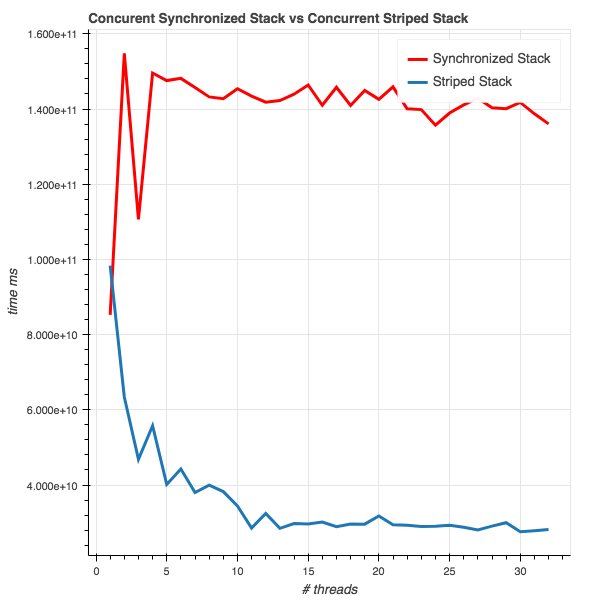
\includegraphics[width=0.7\textwidth]{linkedlist.png}
  \caption{LinkedList vs StripedStack \textit{LinkedList}}
  \label{fig:linkedlist}
\end{figure}

\section{Question 6}

\subsection{Consensus}

Not sure about this but it might be related of the \textit{volatile}, because a read might be interrupted between check and changing the state. 

\begin{lstlisting}[language=java]
volatile int state = -1;
int consensus(int x) { // invariant: x > 0
  assert( x > 0 ) ;
  if( state > 0 )
     return state;
  else
	 state = x;
     return state;
}
\end{lstlisting}

Using a lock based solution using \textit{synchronized} is not wait-free data structure. It might happen that a thread involve unbounded number of retries due to clashes with other threads, thus is not a wait-free and it violates that every consensus protocol has to be wait-free.

\begin{lstlisting}[language=java]
AtomicInteger state = new AtomicInteger(-1);
int consensus(int x) { // invariant: x > 0
    assert( x > 0 ) ;
    if( state.get() > 0 ) return state;
    while( true ) {
        if( state.compareAndSet(-1,x) ) return state.get();
        }   
    }
\end{lstlisting}

This implementation might hang because of the while loop. It might happen that a thread
tries to \textit{compareAndSet} but meantime other thread already change the state, therefore it will fail and will end up in the loop.

\section{Question 7}

\subsection{Akka}

\textit{Implementation SesComSys.java}

\textit{Output}

\begin{lstlisting}[language=java]
Press return to terminate...
public key: 4
private key: 22
cleartext: SECRET
encrypted: WIGVIX
decrypted: SECRET

Press return to terminate...
public key: 18
private key: 8
cleartext: SECRET
encrypted: KWUJWL
decrypted: SECRET

Press return to terminate...
public key: 17
private key: 9
cleartext: SECRET
encrypted: JVTIVK
decrypted: SECRET
\end{lstlisting}


\end{document}
